\section{Introduction}
\label{sec:introduction}


%% \gammaray astronomy
\gammaray astronomy is a rather young field of research. The \gammaray~
range of the electromagnetic spectrum provides us with insight to the
most energetic process in the universe such as surroundings of
black holes and remnants of supernova explosions. As in other
branches of astronomy \gammarays can be observed by both
satellite as well as ground based instruments.
Very high energy cosmic \gammarays reaching Earth interact in the atmosphere and
create a large shower of secondary particles that can be observed from the ground.
Ground-based \gammaray astronomy relies on this phenomenon to detect the
primary \gammaray photons and measure their direction and energy.
It covers the energy range from fews tens of GeV up to the PeV.
There are two main categories of instrument \citep{2015CRPhy..16..610D}.
Imaging Atmospheric Cherenkov Telescopes (IACT) make images of atmospheric showers
by detecting the Cherenkov radiation emitted by the cascading charged particles and
use these images to reconstruct the properties of the incident particle.
Those instruments have a limited field of view (FoV) and duty cycle, but
good energy and angular resolution.

\begin{figure*}[t]
	\centering
	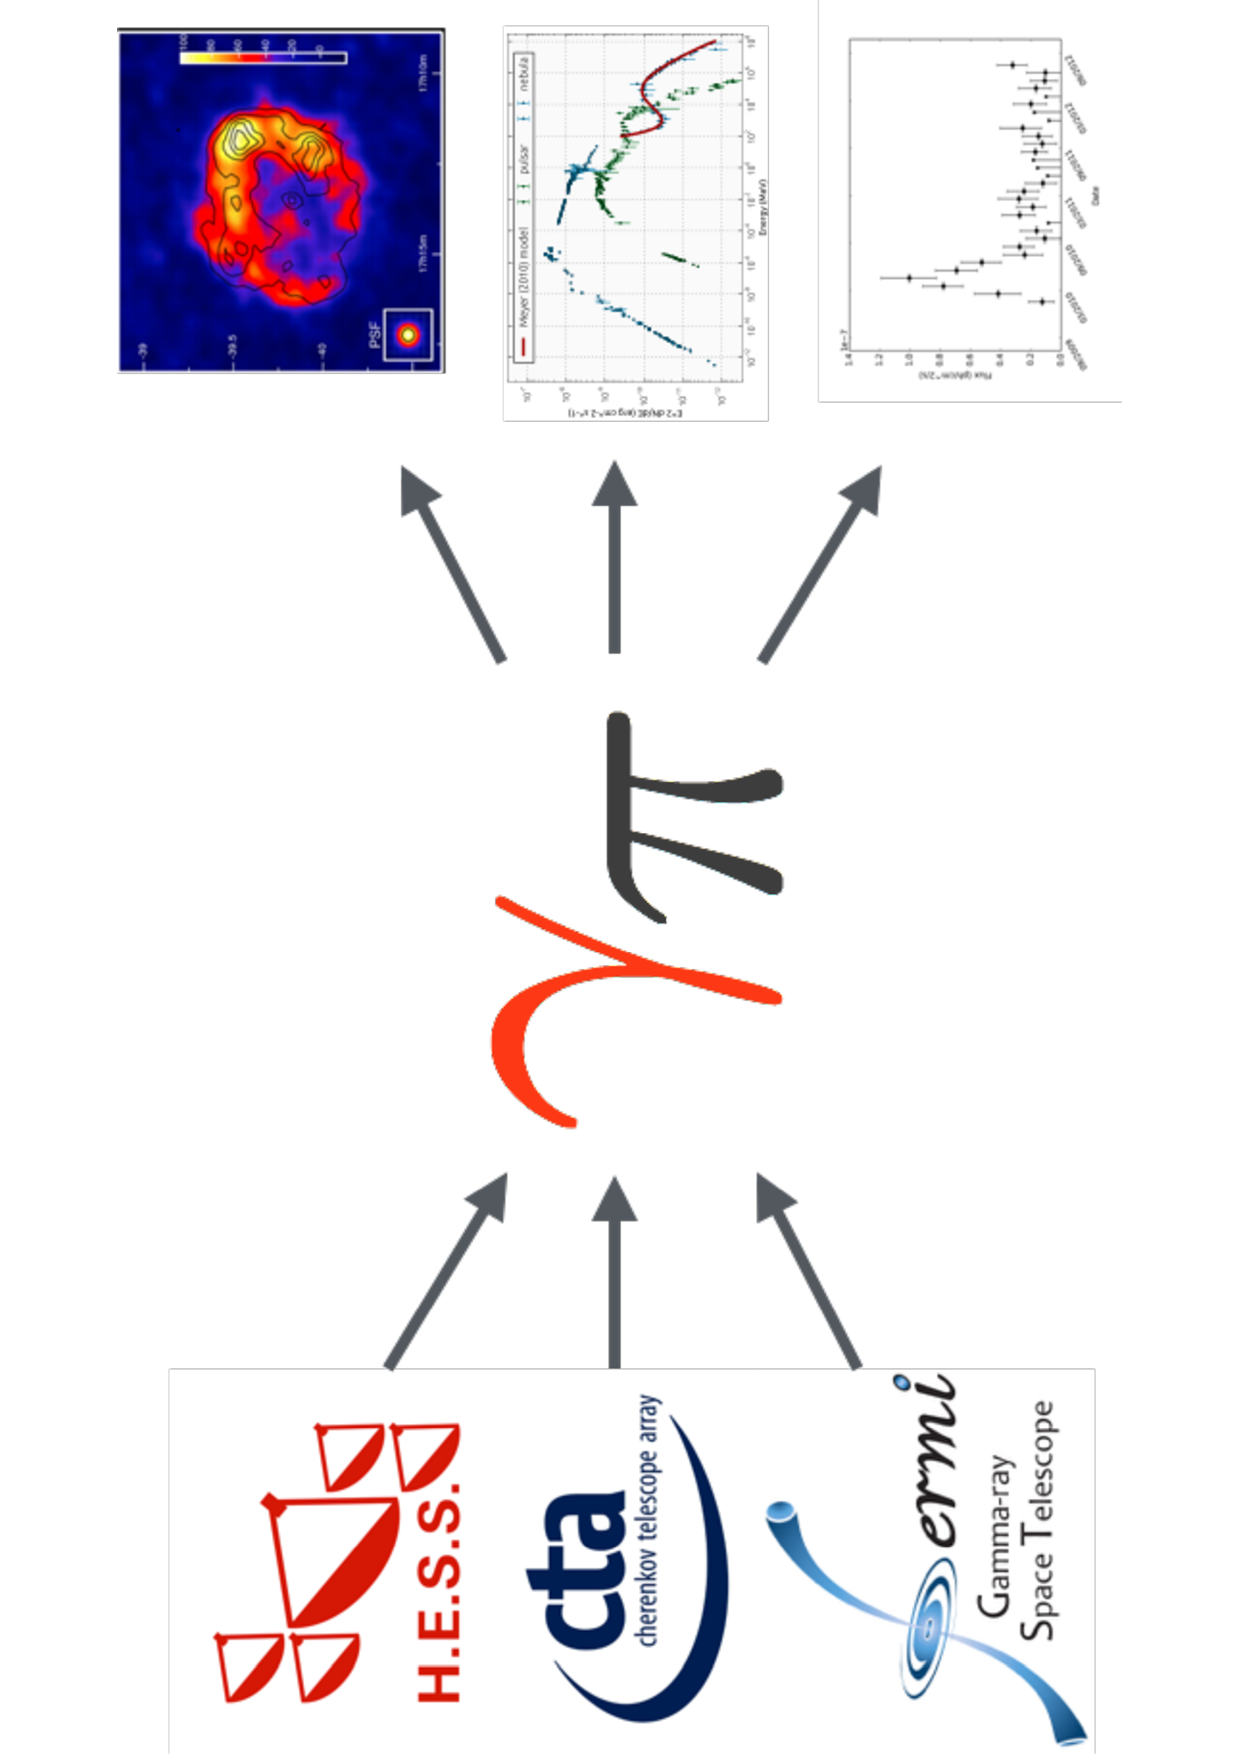
\includegraphics[height=\textwidth, angle=270]{static/gammapy-big-picture}
    \caption{ \gammapy is a Python package
		for high-level \gammaray data analysis. Using event lists, exposures and point
		spread functions as input you can use it to generate science results such as
		images, spectra, light curves or source catalogs. So far it has been used to
		simulate and analyse \hess, \cta,  and \fermi data. As demonstrated
		by several studies, it will also be applied to e.g., \veritas, \magic or \hawc data
		in the future. }
	\label{fig:big-picture}

\end{figure*}

Water Cherenkov observatories detect directly particles from the tail of the
shower when it reaches the ground. These instruments have very
large field-of-view, large duty-cycle but higher energy threshold and
usually have lower signal to noise ratios compared to IACTs.

%% Context
Ground based \gammaray astronomy has been historically structured
by experiments run by independent collaborations relying
on their own proprietary data and analysis software developed as part of the
instrument. While this model has been very successful so far, it does not
permit easy combination of data from several instruments and is therefore
a limitation for interoperability of existing facilities. Especially
because the different detection techniques have complementary
properties.

%TODO: better transition into context
The Cherenkov Telescope Array (CTA) will be the first instrument to be operated
as an open observatory in the domain. Its high level data will be shared publicly after
some proprietary period and the software required to analyze it will be distributed
as well. To allow the re-usability of existing instruments and their interoperability
requires open data formats and open tools that can support the various analysis methods
commonly used in the field.


%% Context : formats
In practice, the data-reduction workflow of all \gammaray observatories
is remarkably similar.
After data calibration, shower events are reconstructed and
gamma/hadron separation is applied to build lists of \gammaray like events.
The latter are then used to derive scientific results, such as spectra, sky maps
or light curves, taking into account the specific instrument response functions (IRF).
The information in this high data level is independent on
the data reduction, and eventually of the detection technique. This implies,
for example, that data from IACT and particle samplers can be represented
within the same model. The efforts to prototype a format usable by various instruments
converged in the so-called \textit{Data Format for \gammaray Astronomy}
initiative~\citep{gadf_proc, gadf_universe}, abbreviated in
\texttt{gamma-astro-data-format} (\gadf). The latter proposes prototypical
specifications to produce files based on the flexible image transport system
(FITS) format~\citep{fits} encapsulating this high-level information. This is
realized by storing a list of gamma-like events with their measured quantites
(energy, direction, arrival time) and a parametrisation of the response of the
system. (see Sec.~\ref{ssec:gammapy-data} and Sec.~\ref{ssec:gammapy-irf} for
more information).

%% Context: develoment of open software
Python has become extremely popular as a scientific programming language
in particular in the field of data sciences. The success is
mostly attributed to the simple and easy to learn syntax, the ability to act as
a "glue" language between different programming languages and last but not least
the rich eco-system of packages and its open and supportive community, from
core numerical analysis packages such as numpy \citep{numpy} and
scipy \citep{2020SciPy-NMeth}, visualization libraries,e.g. matplotlib \citep{matplotlib},
or optimization packages such as iminuit \citep{iminuit}.

The \astropy~\citep{astropy} was created in 2012 to build a community-developed
python package for astronomical reasearch. Among other things, the it offers functionality for
transforming and representing astronomical coordinates, manipulating physical quantities
and their units as well as reading and writing FITS files.

%% \gammapy: concept and goals
%%% Question: starting date? Is is relevant, what is the real start?
The \gammapy project started in 2015 with the objective of building a flexible and
efficient software library for very high energy \gammaray data analysis \citep{gammapy_2015}.
This is possible thanks to the definition of a common data format such as \gadf, and thanks to
an open development with a broad community of contributors.

%\gammapy is built on the scientific Python stack and makes use of Astropy.


%% \gammapy: from first developments to validation and selection
The \hess collaboration released a limited test dataset (about 50 hours of
observations taken between 2004 and 2008) based  on the \gadf DL3 format \citep{HESS_DR1}.
This data release served as a basis for analysis tools validation \cite[see e.g.]{Mohrmann2019}.

TODO: Figure 1: Data -> \gammapy -> Spectra etc with some details

%% Paper outline
In this article, we describe the general structure of the \gammapy package and
its main concepts. In Section \ref{sec:analysis-workflow-overview}, we present
the data analysis workflow in very high energy \gammaray astronomy. Then we
show how this workflow is reflected in the structure of the \gammapy package and
describe the various subpackages it contains. Section \ref{sec:applications}
presents a number of applications, while Section \ref{sec:gammapy-project}
discusses the project organization.


